\chapter{Machine Learning}
\label{chapter:MachineLearning}

\section{Introduction}

As described in Section~\ref{sec:MultiLabelBinaryClassification}, the reconstruct tracks from the reconstructed hits in an event, one must solve a multi-label binary classification problem. This chapter describes how Machine Learning answers this question.

\ \\Since the labels are known, it is a supervised problem. Supervised learning can be either classification or regression. The possibles answers are finite, or categorical, so it is a classification problem. There are several types of classification problems. 

\ \\Multi-class is a classification with more than two classes. In this category each sample is assigned to one and only one label. For example, a color can have only one label from several choices: red, green, blue. In other words, there is only one question, and each answer can be one of three or more labels.

\ \\Multi-label is a classification where each sample is mapped to a set of labels, each being binary. It is as if asking several questions, each with an answer of yes or no. In this case, the question asked for each hit is if the output is -1 or 1 for this hit. So this problem is a multi-label one. 

\ \\The general case is a multi-class multi-label classification problem, when there are many questions, and for each the answer can be chosen from several labels. 

\section{Neural Network Architecture}

Several machine learning algorithms can be used to perform a classification task. The most common are decision trees and neural networks~\cite{AndrewNg}. Several decision trees are trained and grouped together into an enesemble method like random forests and boosted decision trees. In general, to find a multidimensional highly non-linear function representing a non-linear relation between input and output, it is efficient to train a neural network (NN). NNs are statistical models inspired by biological neural networks in the brain. The brain contains millions of neuron cells forming a network where electro-chemical impulses are being passed between them. An artificial neural network is formed by a number of interconnected artificial \emph{neurons}, or \emph{nodes}. In this project NNs are used.

\ \\One of the NN characteristics is that they contain weights along paths between neurons. The weights can be tuned with an algorithms that learns from observed data to improve the model. The NN learns through optimisation techniques, like the gradient descent. A NN is represented by an architecture formed by layers of artificial neurons, which are able to receive several inputs, which are processed by an activation function to determine the output. A simple model is formed by an input layer followed by a hidden layer and then an output layer. Each layer may contain one or more neurons. A NN with more than one hidden layer is called a deep neural network (DNN). For the best DNN performance, the model has to be designed according to the problem to solve, and then hyper-parameters are tuned. A general structure of a fully connected DNN is presented in Figure~\ref{fig:DNN}.

\begin{figure}[h]
  \centering
  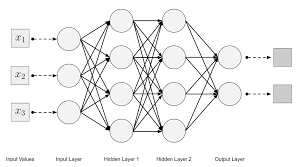
\includegraphics[width=0.6\textwidth]{./plots/DNNArchitecture.png}
  \caption{Diagram of a general architecture of a DNN. Credit image: O'Reilly.~\cite{OReilly}.}
  \label{fig:DNN}
\end{figure}

\ \\The \emph{Universal Approximation Theorem} states that a neural network with one \emph{hidden layer} can in principle approximate any N-dimensional function to an arbitrary degree of accuracy, given a sufficiently large (though finite) number of nodes. In practice however it is more suitable to use multiple hidden layers connected in series~\cite{AndrewNg}.

\ \\In a fully connected NN, each node takes a weighted linear combination of the outputs from nodes of the previous layer, adds its own bias value, and applies an \emph{activation function}, then outputs the result to the neurons of the next layer, as illustrated in Figure~\ref{fig:Neuron}. The activation function is choosen via optimisation for each neuron when the architecture of the NN is defined. 

\begin{figure}[h]
  \centering
  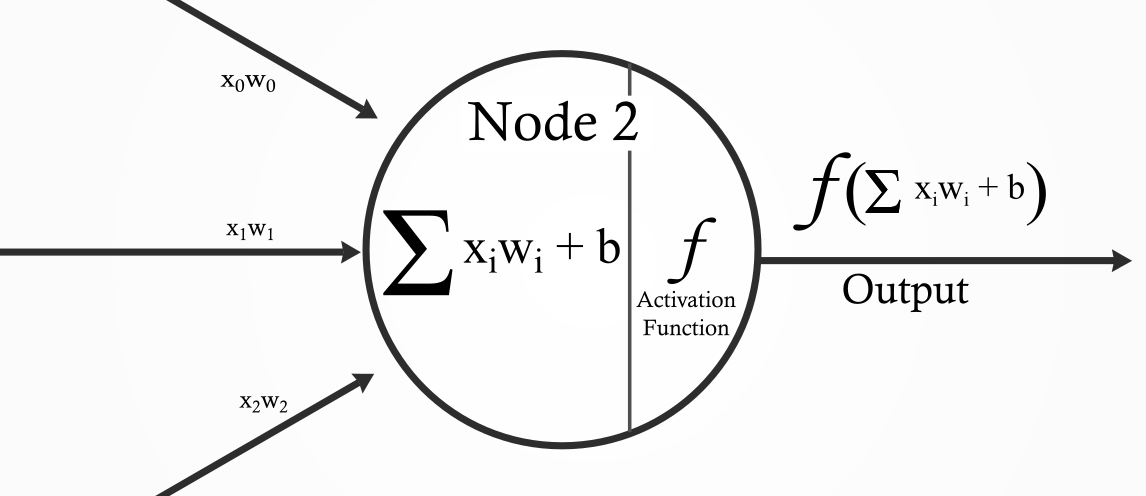
\includegraphics[width=0.6\textwidth]{./plots/Neuron.png}
  \caption{Diagram of a neuron or node in a NN, with its weight inputs, its bias and the output via the activation function. Credit image: The Fork~\cite{TheFork}.}
  \label{fig:Neuron}
\end{figure}

\ \\Once the NN architecture is set, the layers, nodes and activation functions, the total function of the NN is parametrized by all the weights for the connections between nodes plus the biases of each node. Training the NN means learning these weights and biasis so that the NN function can predict well the output when a new data not seen before is taken as input.

\section{Hyper-Parameters}
\label{sec:Hyperparameters}

Several hyper-parameter choices can be made depending on the question being asked, regarding the number of hidden layers, number of nodes on a hidden layer, the activation function of nodes in the hidden layers, the activation function of nodes in the output layer, the learning optimizer, the loss function, the batch size. In the plots of this section the hyper-parameters that are retained for the best performing model are colored in red, to already ilustrate their behaviour relative to the other possible hyper-parameters.

\ \\The problem is a multi-label binary classification. Given a collection (bucket) of 20 hits, for each hit there is a question of a binary classification (if yes or no) the hit belongs to the particle with the largest number of hits in the bucket. 

\ \\The output labels of yes and no may be encoded as 1.0 and 0.0, or as 1.0 and -1.0, respectively. A preliminary study suggests that the latter option provides better results. With this choice, there remains only a limited choice of activation functions of the output layer and of loss functions. 

\ \\Firstly, the output value of the NN prediction fixes the choice of the activation function on the last layer to the hyperbolic tangent (TANH), which has values between -1.0 and 1.0, and not the logistic regression, also called sigmoid, which has values between 0.0 and 1.0, illustrated in Equations

\begin{equation}
   \tanh x = \frac{\sinh x}{\cosh x} = \frac{e^x - e^{-x}}{e^x + e^{-x}} = \frac{e^{2x}-1}{e^{2x}+1}
\end{equation}

\ \\and

\begin{equation}
   S(x) = \frac{1}{1 + e^{-x}} = \frac{e^{x}}{e^{x}+1}.
\end{equation}

\ \\and on the left-hand side of Figure~\ref{fig:ActivationFunctionsLastLayer}. Two more activation functions are possible for values between -1.0 and 1.0. The square non linear (SQNL) is described by Equation

\begin{equation}
   \SQNL~(x) = 
\begin{dcases}
    -1 , & x < -2.0\\
    x + \frac{x^2}{4}, & -2.0 \leq x < 0\\
    x - \frac{x^2}{4}, & 0 \leq x < 2.0\\   
    1 , & x > 2.0\\
\end{dcases}.
\end{equation}

\ \\ and the soft sign (SOSI) function by Equation

\begin{equation}
   \SOSI~(x) = \frac{x}{1 + |x|}.
\end{equation}

\ \\All three functions reach the values of -1.0 and 1.0, but for different values of x. SQNL, TANH and SOSI reach the value of 1.0 (-1.0) for the x values of exactly 2.0 (-2.0), of around $\pi \sim 3.14$ (-$\pi \sim -3.14$) and for $\infty$ ($-\infty$), respectively, as illustarted in the right-hand side of Figure~\ref{fig:ActivationFunctionsLastLayer}.

\begin{figure}[htb]
\centering
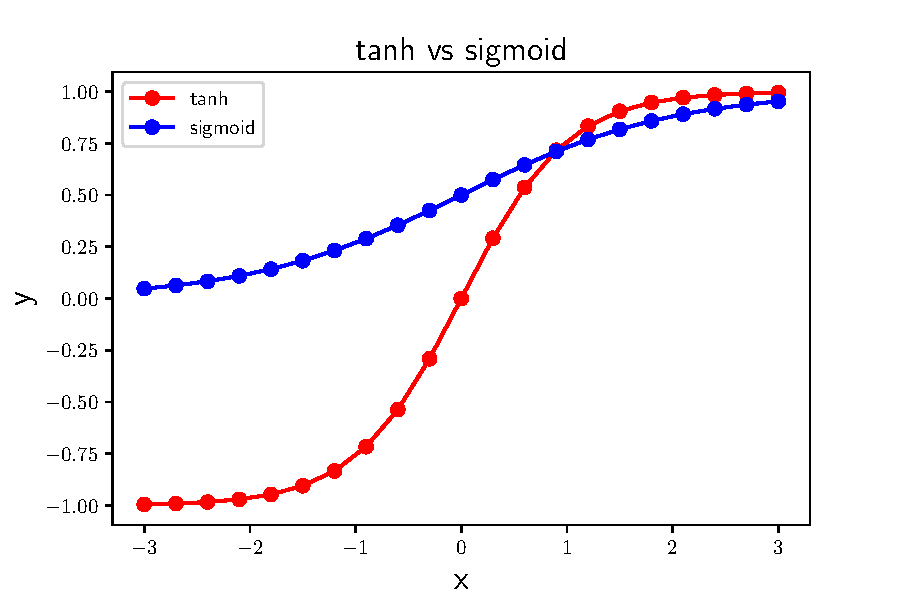
\includegraphics[width=0.45\textwidth]{plots/ActivationFunctionsLastLayer1.pdf}
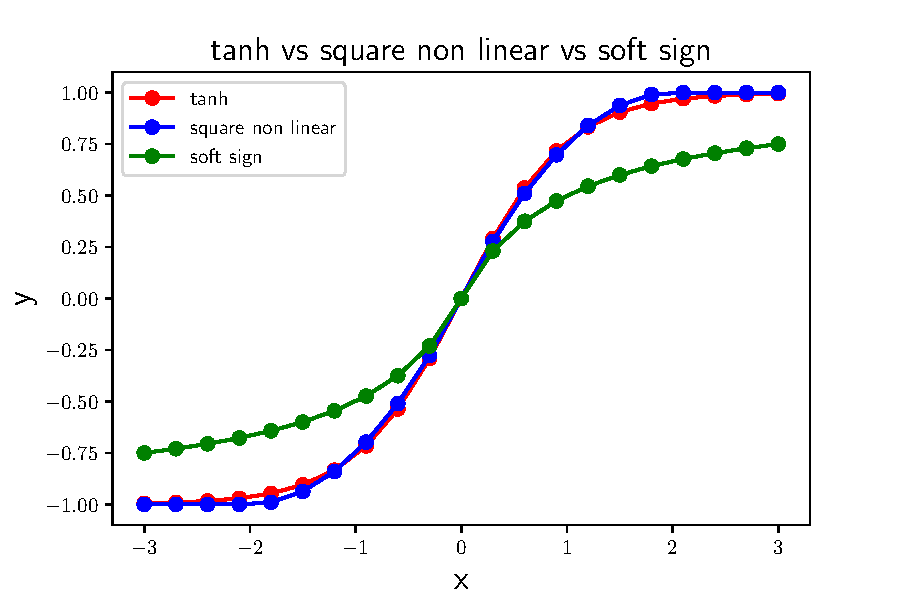
\includegraphics[width=0.45\textwidth]{plots/ActivationFunctionsLastLayer2.pdf}
\caption{Overlaid potential activation functions for the last layer. Left: hyperbolic tangent (tanh) and logistic regression (sigmoid). Right: tanh, square non linear and soft sign. Tanh is chosen as our output labels are -1.0 and 1.0.}
\label{fig:ActivationFunctionsLastLayer}
\end{figure}

\ \\The appropriate loss functions for the target values of -1.0 and 1.0 are only the (regular) hinge function and the squared hinge function. Denoting y the predicted output and t the true target output (label), the hinge function is given by the Equation

\begin{equation}
   \LossFunctionHinge:~l(y) =  \max(0, 1 - t \cdot y),
\end{equation}

\ \\and the squared hinge by the Equation

\begin{equation}
   \LossFunctionSquaredHinge:~l(y) = [\max(0, 1 - t \cdot y)]^2.
\end{equation}

\ \\Their relative behaviour is illustrated in Figure~\ref{fig:LossFunctions} for t=-1.0 (left) and t=1.0 (right). These loss functions never become negative. For t=1.0, for $y \ge t$, the loss function is exactly zero. For $y<t$, the loss function gradually increases. The squared hinge does not have a discontinuity at $y=1$ and at high values increases more than the regular hinge, penalizing large deviations more. The same is valid for y=-1.0, but in the opposite direction. 

\begin{figure}[htb]
\centering
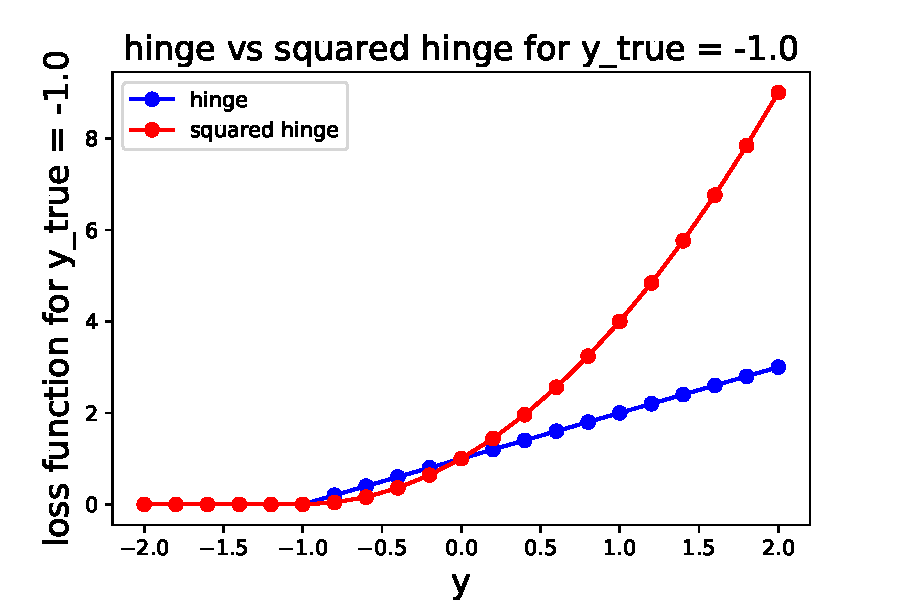
\includegraphics[width=0.45\textwidth]{plots/LossFunctions_MinusOne.pdf}
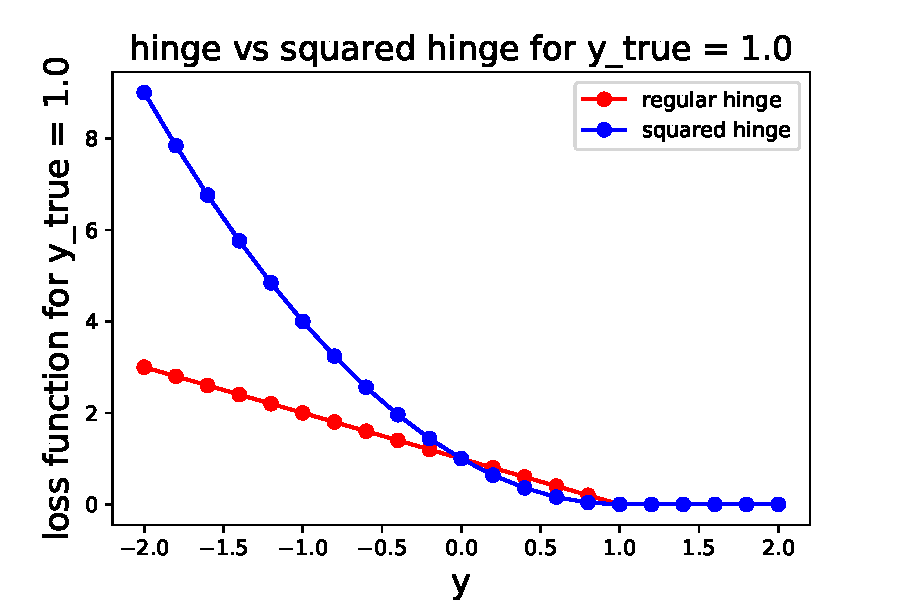
\includegraphics[width=0.45\textwidth]{plots/LossFunctions_PlusOne.pdf}
\caption{Overlaid loss functions of (regular) hinge and squared hinge for varying predicted y, for a fixed true y of -1.0 (left) and 1.0 (right).}
\label{fig:LossFunctions}
\end{figure}

\ \\The functions above apply to a pair of predicted y and true t values. In our problem it refers to each hit. The final loss function for the entire sample represents a sum over all the buckets in all events in the train or test sample, and for each bucket the sum over each of the 20 hits, as exemplified in Equation

\begin{equation}
   \LossFunctionHinge:~l(y) = \sum_{\rm bucket} \sum_{\rm hit} \max(0, 1 - t_{\rm hit} \cdot y_{\rm hit})
\end{equation}

\ \\ and

\begin{equation}
   \LossFunctionSquaredHinge:~l(y) = \sum_{\rm bucket} \sum_{\rm hit} [\max(0, 1 - t_{\rm hit} \cdot y_{\rm hit})]^2.
\end{equation}

\ \\Another choice to make is that of the activation functions for the nodes of the hidden layers. Besides the already-mentioned sigmoid and hyperbolic tangent functions, the Rectified Linear Unit (ReLU) is introduced. ReLU is the mostly common activation function for neural networks nowadays, including for more advanced neural networks such as convolutional neural networks (CNN) or deep neural networks (DNN). ReLU is \emph{rectified} from the bottom, meaning its values are zero for negative inputs and return the same value as the input for positive inputs. ReLU can be summarized by Equation

\begin{equation}
   \ReLU:~R(x)= \max(0, x).
\end{equation}

\ \\While both the function R(x) and its derivative are monotonous, the function also has some drawbacks. is not differentiable at zero. Since for all negative values the input is exactly zero, for methods learning with gradient descent, the ability to learn is reduced. To address this problem, a variation of ReLU is introduced, namely and the Exponential Linear Function (ELU), described by Equation

\begin{equation}
     \ELU:~E(x= 
\begin{dcases}
    \alpha(e^x -1), & x < 0\\
    x,              & x \geq 0
\end{dcases}.
\end{equation}

\ \\For positive values, the function remains the same. But for the negative values, an exponential curve appears, tending smoothly to a constant value $\alpha$. ELU has the advantage over ReLU to be fully continuous and differentiable, and not having a vanishing gradient problem for gradient descent learning. Its main disadvtange is that it is slower to compute for negative values. But it may be worth it for a more precise result. The comparison of the ReLU and ELU functions is illustrated in Figure~\ref{fig:ActivationFunctionsHiddenLayers}.

\begin{figure}[htb]
\centering
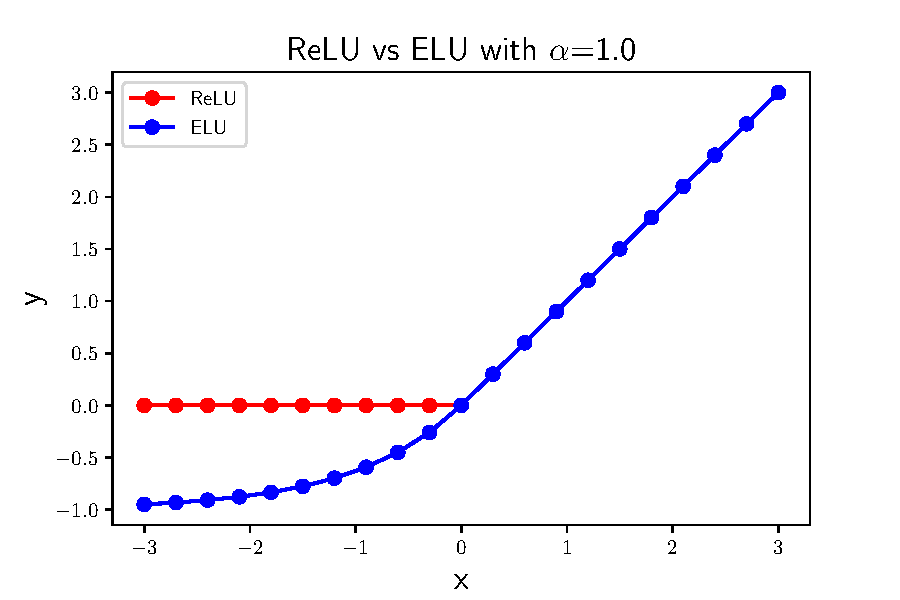
\includegraphics[width=0.45\textwidth]{plots/ActivationFunctionsHiddenLayers.pdf}
\caption{Overlaid activation functions of ReLU and ELU, with $\alpha=1.0$.}
\label{fig:ActivationFunctionsHiddenLayers}
\end{figure}

\ \\Another hyper-parameter to tune is the number of hidden layers and the number of nodes on each hidden layer. The \emph{Universal Approximation Theorem} suggests that one layer with a very large number of nodes is enough to learn any arbitrary function. But in practice it is worth having several consecutive layers of fewer nodes per layer. That forms a deep neural network. 

\ \\Another option in the architecture of the NN is whether to use or not to add a regularisation layer, in particular a dropout layer~\cite{DropoutLayer}. Sometimes the resulting model is too complex relative to the quantity of input data, leading to overfitting during training. Overfitting is similar to memorisation of the input data, leading to not be able to predict correctly on new data. To avoid overfitting, regularisation techniques are used. Typical methods add a new term to the loss functions. Other techniques add a dropout layer. The dropout method sets randomly some of the inputs to 0 with a frequency $f$, and reweights the other inputs by $1/(1-f)$, so that the total sum of inputs remains constant. The value of $f$ is a hyper-parameter to be optimised. The location of the dropout layer is usually between the hidden layers and the last layer. Dropout is applied only during training, and not during testing or infering on new data.

\ \\Another choice related to the learning method is the learning optimiser. Two algorithms based on stochastic gradient descent are compared, namely Adam~\cite{Adam} and AdaDelta~\cite{AdaDelta}. For both their default parameters are used, the most important being the learning rate of 0.001. Adam is very computationally efficient, while AdaDelta uses adaptive learning rate. 

\section{Learning Methods}

NN training is done learning on the training dataset and testing on the testing dataset. Running once over all the data from training and testing represents an \emph{epoch}. During an epoch, events are analysed in groups called \emph{batches}. The number of epochs to run on and the number of events in each batch can be optimised.

\ \\ Let's take a look at how the NN training happens. At first the NN has random values for the weights and biases. For each of the events in the first batch, data comes in, and the NN predicts an output values, that are at first very different from the true desired output value. To evaluate how far away are the predicted output from the desired output, a \emph{loss} function is defined that can be chosen from several formulas, but have the generic form of a sum over the absolute values of these differences. The goal of the NN training is to update the values of the weights and biases so that the loss function is minimized. After the first batch, the NN changes the weights via a back-propagation aglorithm using the optimiser algorithm. For each new batch, the weights and biases change, and become continously closer to the correct values, as the loss function becomes gradually smaller. When all the training events are used, the first epoch is finished. The NN function at this point is then applied to the new dataset from the testing dataset, which is not split in batches, and a loss function is also calculated. The entire procedure repeats for the number of epochs chosen. At the end, the final weights and biases define the final NN model that has been learned.

\section{Train and Test Split and k-fold}
\label{sec:TrainAndTest}

The k-fold validation is a procedure used to test the effectiveness of a machine learning model. It is used especially if the data are limited. Normally, the data are split in two equal parts (train and test), corresponding to k=2. For a general k, the data are split randomly into k groups. k-1 groups are used in training and the last one in testing. The operation is repeated by permuting the groups, so that each group is used only once in testing. The final result is obtained by averaging out the permutations.

\ \\It is also possible to split into two unequal parts. In this project the split is done with k=2, 70\% in train and 30\% in test. Although teach data sample is a bucket, it is convenient to use that events have about the same number of buckets. The split of 100 events is done with 70\% of events in train and 30\% of events in test. One can split the events randomly, as by the laws of particle physics events simulate independent particle collisions. NN training takes a significant amount of time. It is useful to train on an increasing data sample size and check if the performance reaches a plateau. For convenience, to study easily with a step of 10 events, events are grouped in consecutive order by 10, with the first 7 events being used for training (Train sample) and the following 3 events are used for testing (Test sample). The pseudo-code is described in Appendix~\ref{sec:AppendixPseudoCodeInputOutput}.

\section{Balancing Datasets}
\label{sec:BalancingDatasets}

It is common practice in ML classification problems that the signal target is much rarer than the backgrounds. It is said the dataset is unbalanced. The solution is to balance the dataset by increasing the weights of signal events such that the total sum of weights of signal equals the total sum of weights for background. The NN learning uses for each data samples its own specific weight. A balanced dataset is used for training. It is not used in testing, in order to represent a real-world situation when one tries to predict the proportion of signa to background, and does not know the balancing ratio. 

\ \\This project involves a multi-label classification problem, where there are 20 hits in a bucket, and for each hit a classification question is asked, if it is a signal (1) or background (0) relative to being part of the majority particle in the bucktet. From physics studies in Chapter~\ref{chapter:TrackML}, it is decided that all buckets with less than 10 hits with output = 1, have all their hits set to output = -1. The dataset becomes even more unbalanced. Balancing is done in two steps.

\ \\First, buckets are removed so that there are equal number of buckets for each of \nbPositiveHit\ between 10 and 17. Values 18-20 are left unchanged, as they are too small. The goal is to learn uniformly and not be biased towards a particular category. \nbPositiveHit~between 1 and 9 are zero by constructions, as all these values are moved to \nbPositiveHit~of zero, which originally did not have any entries. Then the number of buckets of \nbPositiveHit=0 is reduced so that overall, there are exactly equal numbers of positive and negative hits in the sample. That ensures the most general way for learning, without a bias towards one category or the other. The training set is balanced, keeping about 130k buckets. The testing set remains unbalanced, with roughly 3.2M bckets.

\section{Hyper-Parameter Tuning}
\label{sec:HyperparameterTuning}

The hyper-parameters are tuned by choosing the models that perform best in the test sample over 300 epochs, looking at the accuracy and loss that result directly from Keras/TensorFlow after the training. In the plots of this section, the best model summarised in Section~\ref{sec:BestModel} is compared with alternative models where all hyper-parameters are kept constant, except one that is changed. Since training on 1200 epochs and an unbalanced test dataset takes too long, 300 epochs and the balanced test dataset are used. The balanced train dataset are used both in this study and for the final result with 1200 epochs, described in Chapter~\ref{chapter:ModelPerformance}. From this study the best performining hyper-parameters are chosen. When the performance of several hyper-parameters is similar, the simplest or most commonly used hyper-parameter is chosen. The resulting final model is presented in Section~\ref{sec:BestModel}.

\subsection{DNN Architecture}
\label{sec:DNNArchitecture}

A comparison of the number of hidden layers is studied. The performance is similar for different values, and 3 hidden layers is retained for the final model, as it provides a slightly better performance, as illustrated in Figure~\ref{fig:HPNbHiddenLayers}.

\begin{figure}[htb]
\centering
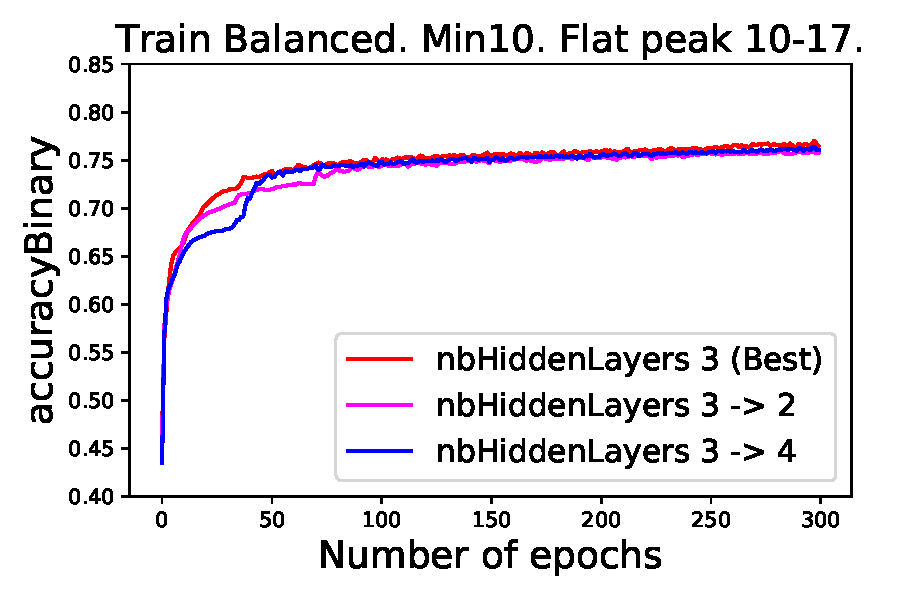
\includegraphics[width=0.32\textwidth]{plots/plot_01_1_overlay_graph_accuracyBinary_Train_NbHiddenLayers.pdf}
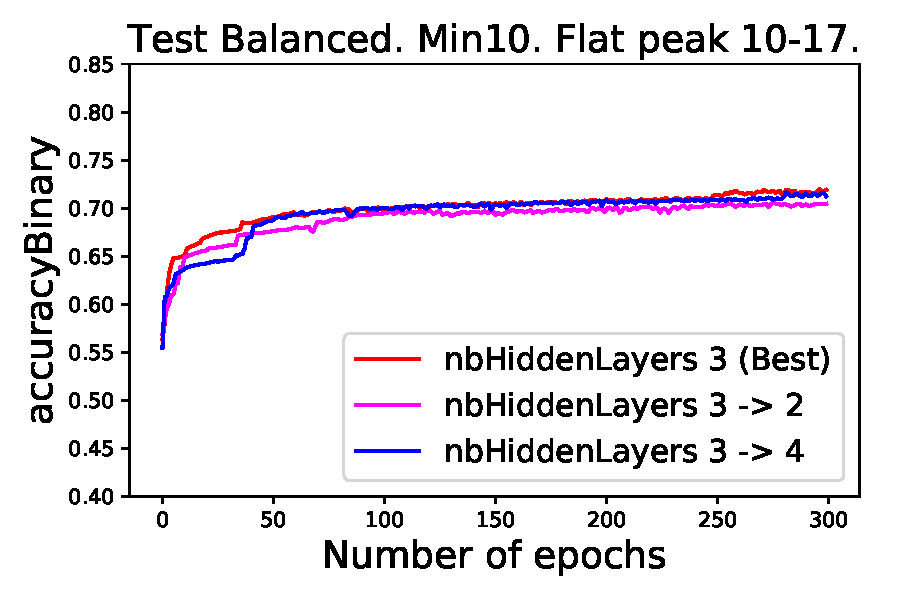
\includegraphics[width=0.32\textwidth]{plots/plot_01_1_overlay_graph_accuracyBinary_Test_NbHiddenLayers.pdf}\\
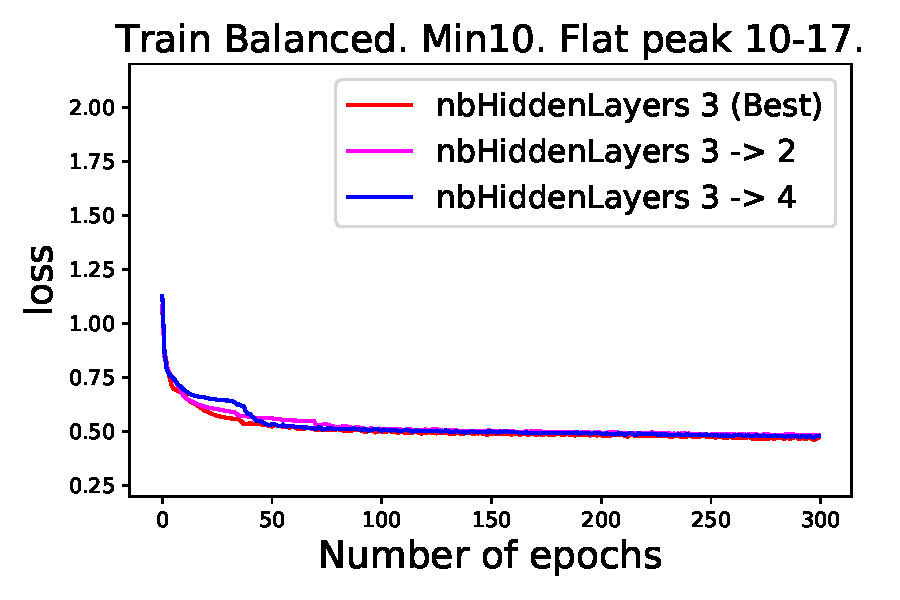
\includegraphics[width=0.32\textwidth]{plots/plot_01_1_overlay_graph_loss_Train_NbHiddenLayers.pdf}
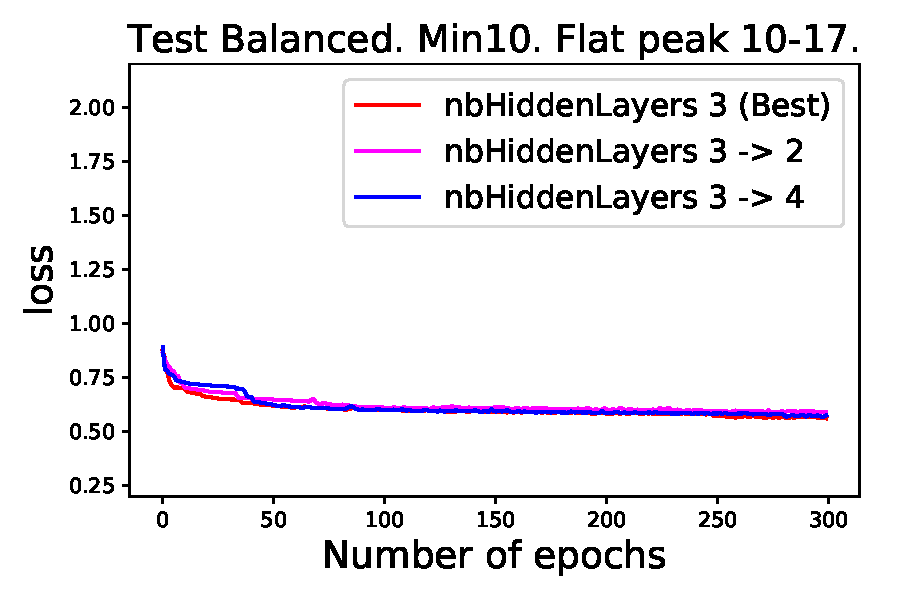
\includegraphics[width=0.32\textwidth]{plots/plot_01_1_overlay_graph_loss_Test_NbHiddenLayers.pdf}\\
\caption{Comparison of different numbers of hidden layers. 3 hidden layer is best. Binary accuracy and loss in Train and Test balanced samples.}
\label{fig:HPNbHiddenLayers}
\end{figure}

\ \\A comparison of the number of nodes on the hidden layers is studied. For simplicity, in this study it is considered the same number of nodes on each hidden layer. The performance is similar for different values, and 200 nodes on the hidden layers is retained for the final model, as illustrated in Figure~\ref{fig:HPNbNodesOnHiddenLayers}. This represents 10 times more than the nodes on the output layer.

\begin{figure}[!htb]
\centering
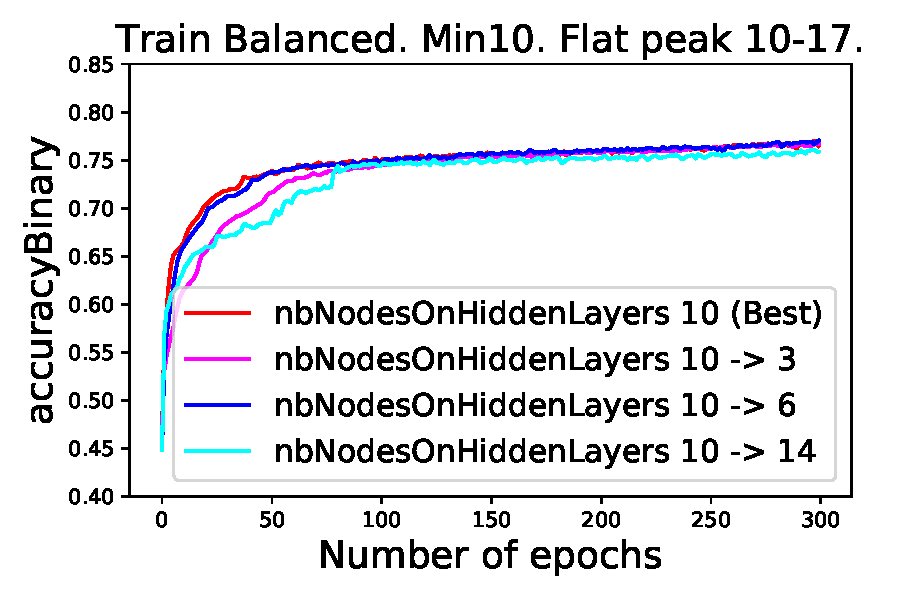
\includegraphics[width=0.32\textwidth]{plots/plot_01_1_overlay_graph_accuracyBinary_Train_NbNodesOnHiddenLayers.pdf}
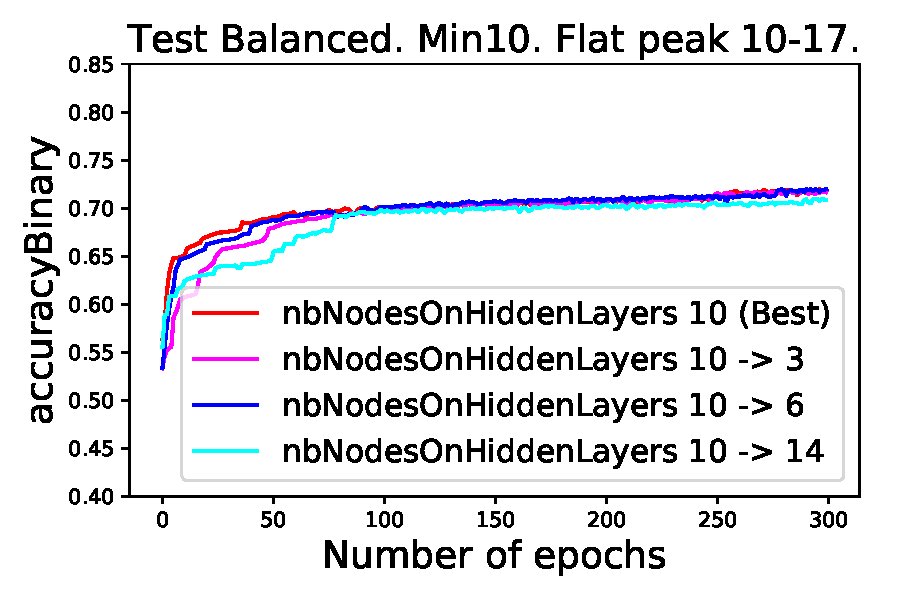
\includegraphics[width=0.32\textwidth]{plots/plot_01_1_overlay_graph_accuracyBinary_Test_NbNodesOnHiddenLayers.pdf}\\
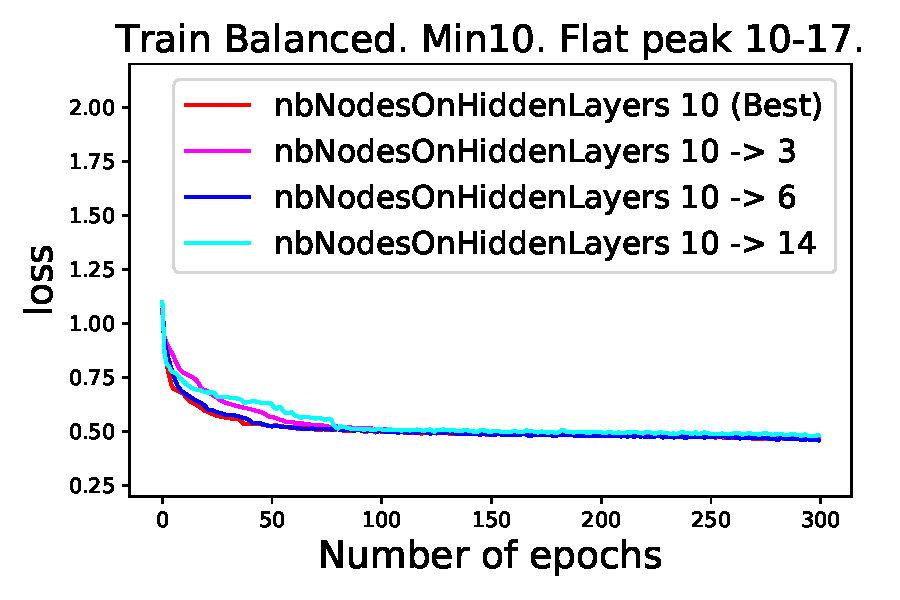
\includegraphics[width=0.32\textwidth]{plots/plot_01_1_overlay_graph_loss_Train_NbNodesOnHiddenLayers.pdf}
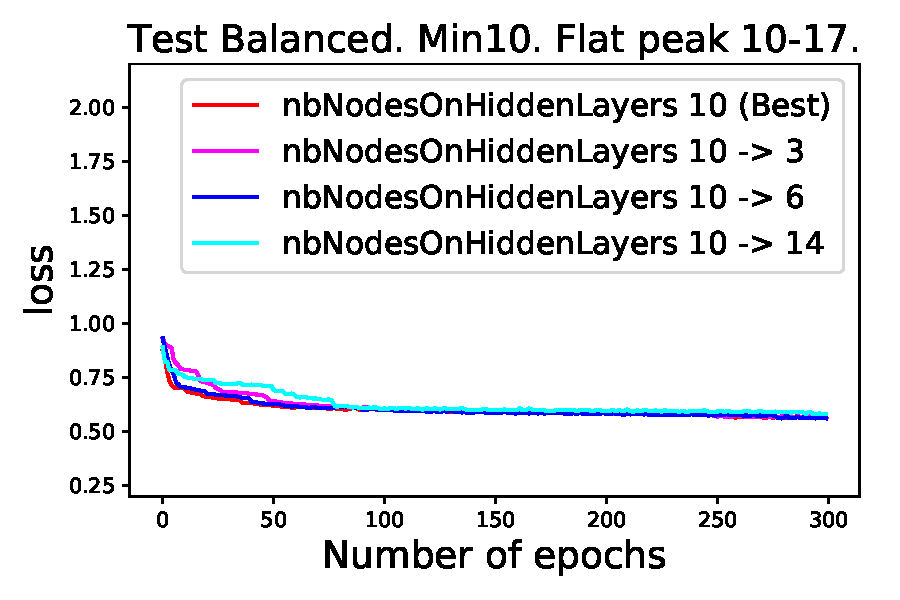
\includegraphics[width=0.32\textwidth]{plots/plot_01_1_overlay_graph_loss_Test_NbNodesOnHiddenLayers.pdf}\\
\caption{Comparison of the ratio of the different number of nodes on the hidden layers divided by the number of nodes on the last layer. k=10, or 200 nodes on each hidden layer, is best. Binary accuracy and loss in Train and Test balanced samples.}
\label{fig:HPNbNodesOnHiddenLayers}
\end{figure}

\ \\A comparison of the activation functions for the hidden layers, namely ReLU and ELU, is performed. For simplicity, in this study it is considered that all nodes of all hidden layers have the same activation function. The performance is similar between the two options, so the standard and mostly used ReLU is retained for the final model, as illustrated in Figure~\ref{fig:HPActivationFunctionHiddenLayers}.

\begin{figure}[!htb]
\centering
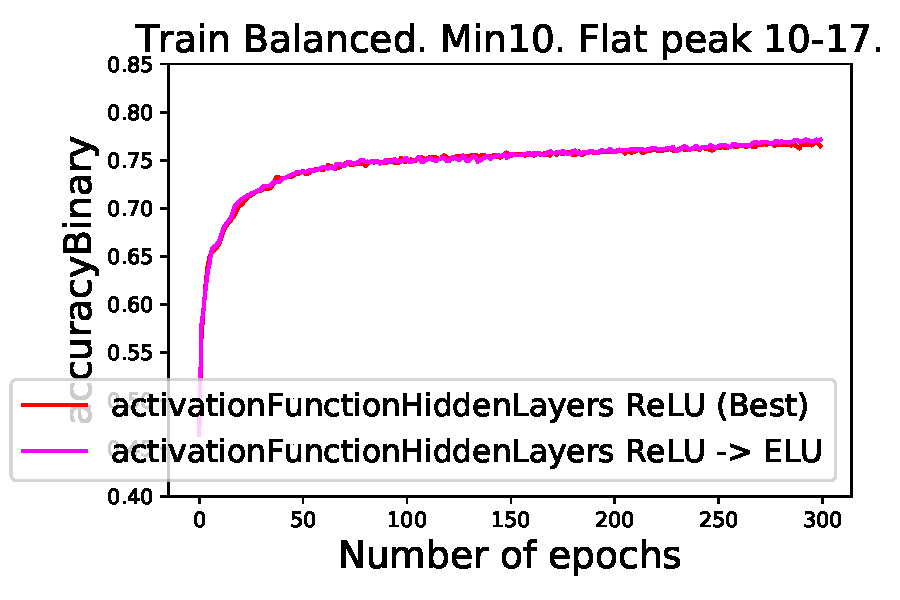
\includegraphics[width=0.32\textwidth]{plots/plot_01_1_overlay_graph_accuracyBinary_Train_ActivationFunctionHiddenLayers.pdf}
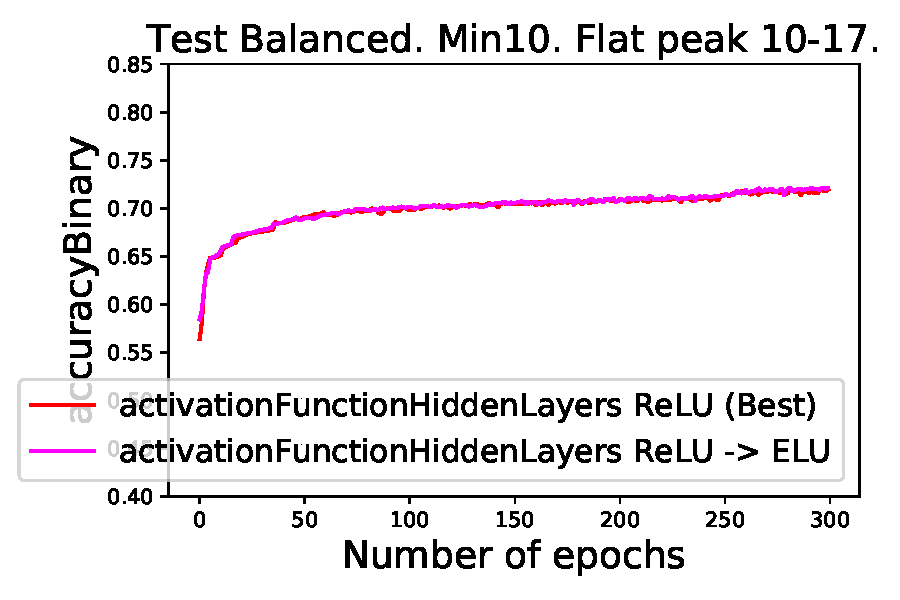
\includegraphics[width=0.32\textwidth]{plots/plot_01_1_overlay_graph_accuracyBinary_Test_ActivationFunctionHiddenLayers.pdf}\\
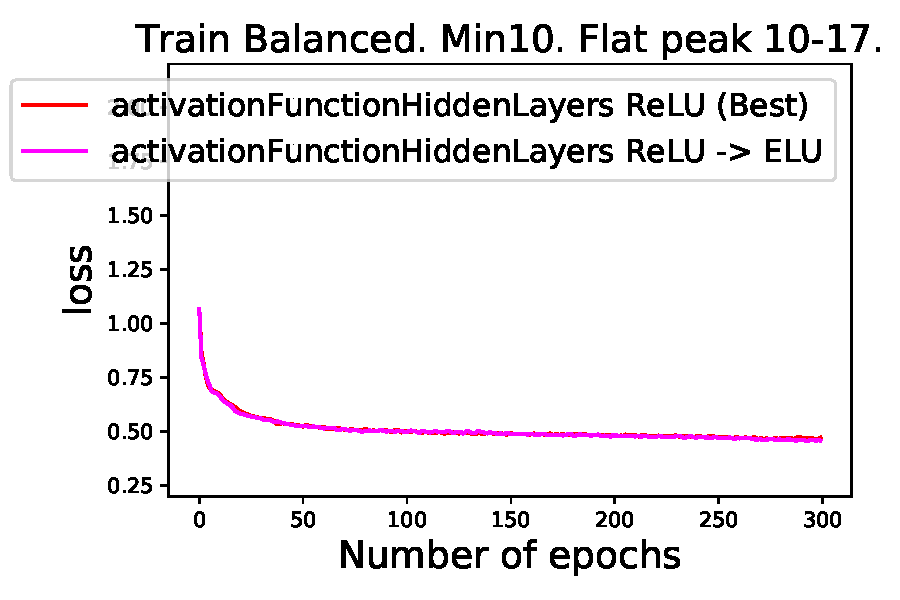
\includegraphics[width=0.32\textwidth]{plots/plot_01_1_overlay_graph_loss_Train_ActivationFunctionHiddenLayers.pdf}
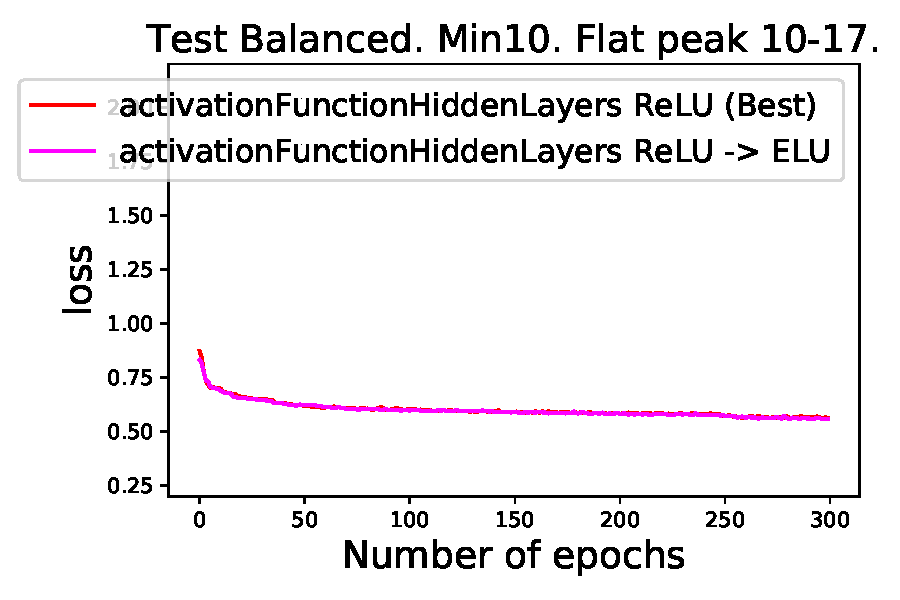
\includegraphics[width=0.32\textwidth]{plots/plot_01_1_overlay_graph_loss_Test_ActivationFunctionHiddenLayers.pdf}\\
\caption{Comparison of ReLU and ELU activation functions on the hidden layers. ReLU is chosen for the final model. Binary accuracy and loss in Train and Test balanced samples.}
\label{fig:HPActivationFunctionHiddenLayers}
\end{figure}

\ \\A comparison of adding or not adding a regularisation function via the dropout layer at the end of the hidden layers is studied. The performance is better by having a dropout layer, as illustrated in Figure~\ref{fig:HPDropoutLayer}.

\begin{figure}[!htb]
\centering
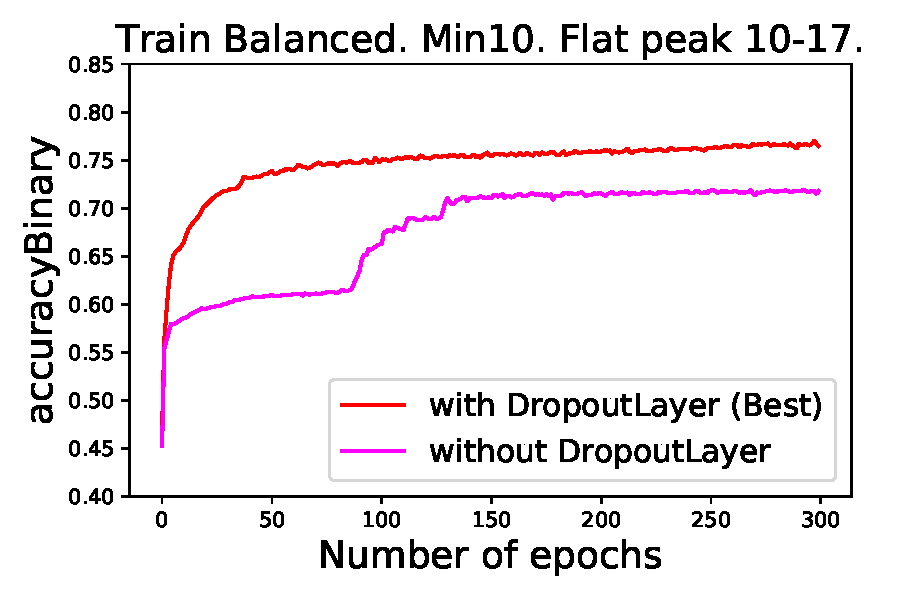
\includegraphics[width=0.32\textwidth]{plots/plot_01_1_overlay_graph_accuracyBinary_Train_DropoutLayer.pdf}
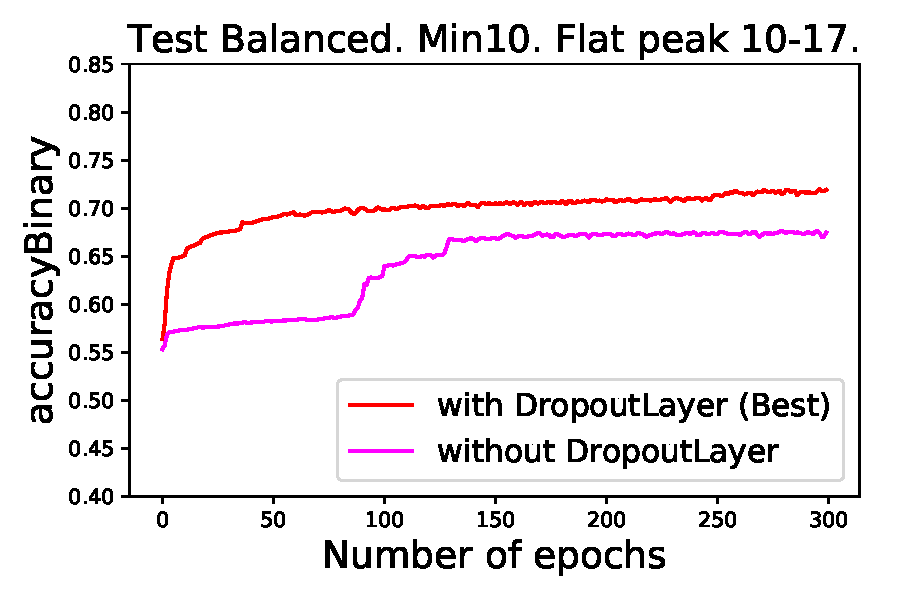
\includegraphics[width=0.32\textwidth]{plots/plot_01_1_overlay_graph_accuracyBinary_Test_DropoutLayer.pdf}\\
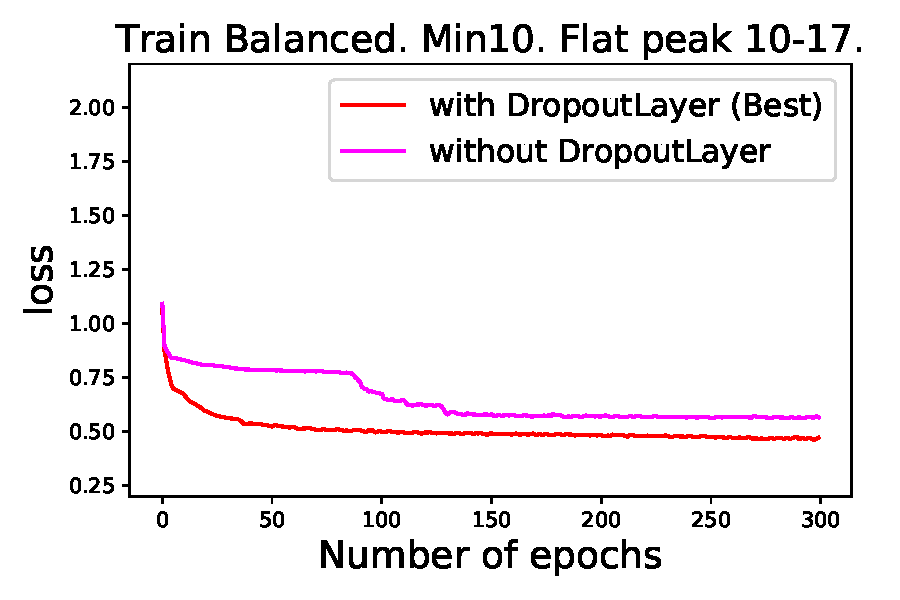
\includegraphics[width=0.32\textwidth]{plots/plot_01_1_overlay_graph_loss_Train_DropoutLayer.pdf}
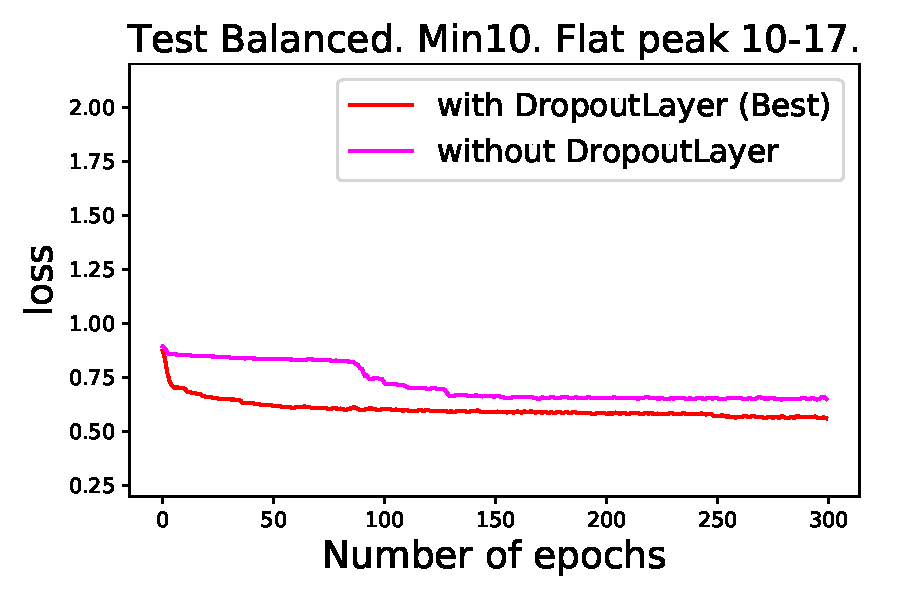
\includegraphics[width=0.32\textwidth]{plots/plot_01_1_overlay_graph_loss_Test_DropoutLayer.pdf}\\
\caption{Comparison without and with a dropout layer for regularisation. A dropout layer is used in the final model. Binary accuracy and loss in Train and Test balanced samples.}
\label{fig:HPDropoutLayer}
\end{figure}

\ \\A comparison of the activation functions for the last layer, namely TANH, SQNL and SOSI, is studied. The performance is similar for the three options, so the standard and mostly used TANH is retained for the final model, as illustrated in Figure~\ref{fig:HPActivationFunctionLastLayer}.

\begin{figure}[!htb]
\centering
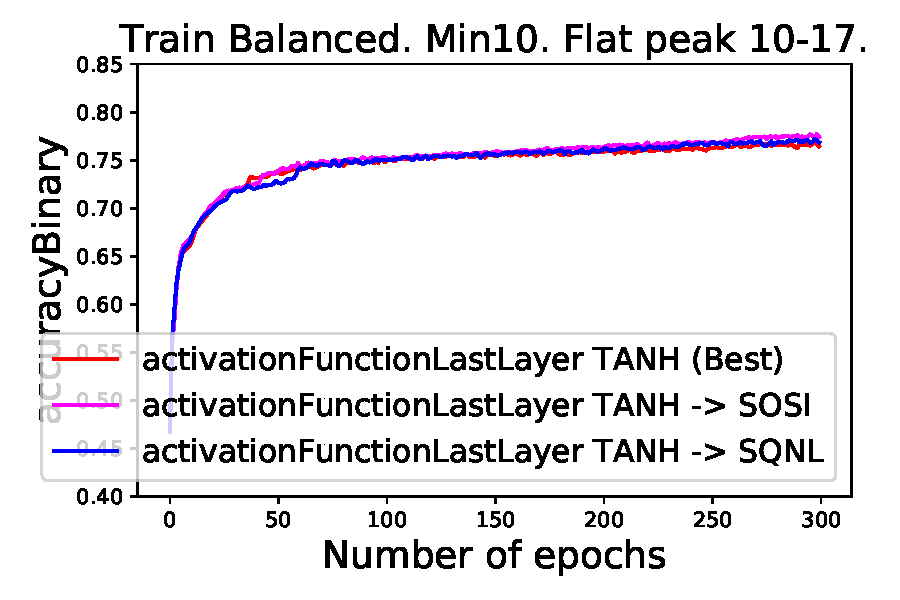
\includegraphics[width=0.32\textwidth]{plots/plot_01_1_overlay_graph_accuracyBinary_Train_ActivationFunctionLastLayer.pdf}
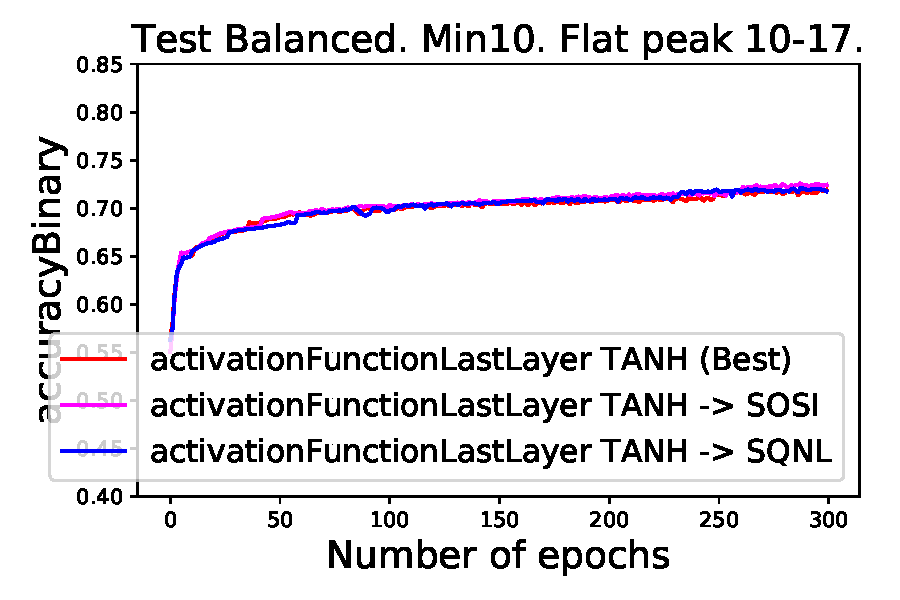
\includegraphics[width=0.32\textwidth]{plots/plot_01_1_overlay_graph_accuracyBinary_Test_ActivationFunctionLastLayer.pdf}\\
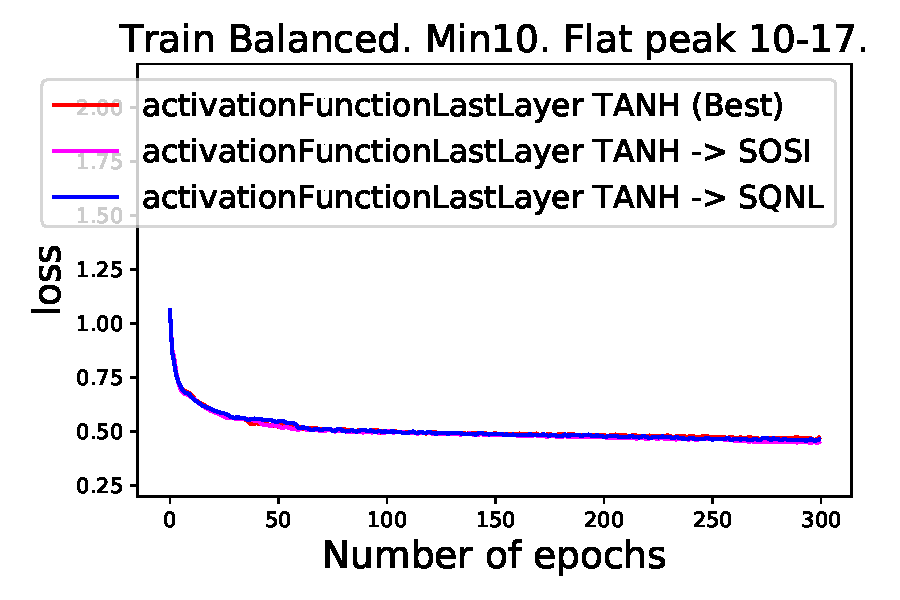
\includegraphics[width=0.32\textwidth]{plots/plot_01_1_overlay_graph_loss_Train_ActivationFunctionLastLayer.pdf}
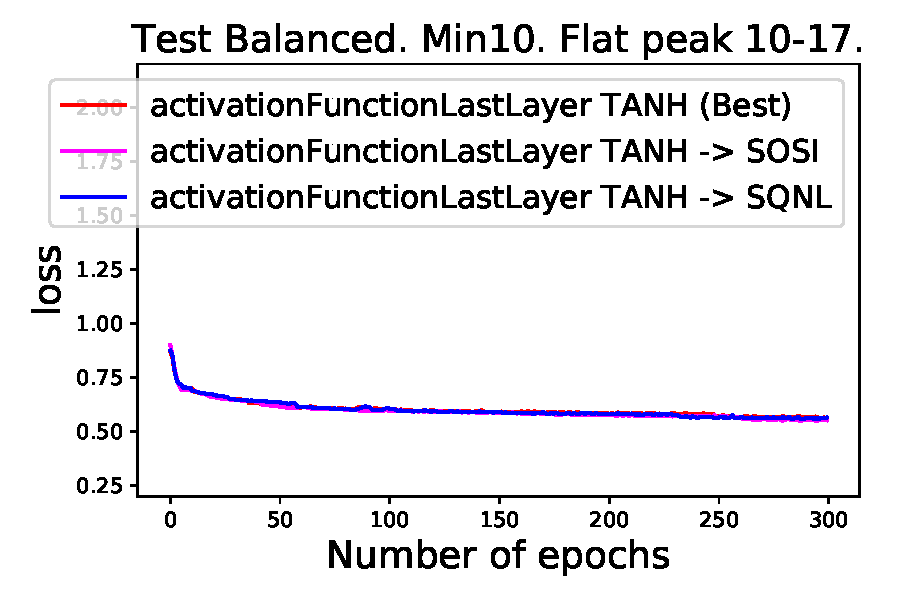
\includegraphics[width=0.32\textwidth]{plots/plot_01_1_overlay_graph_loss_Test_ActivationFunctionLastLayer.pdf}\\
\caption{Comparison of TANH, SQNL and SOSI as activation functions on the last layer. TANH is used in the final model. Binary accuracy and loss in Train and Test balanced samples.}
\label{fig:HPActivationFunctionLastLayer}
\end{figure}

\subsection{DNN Learning}
\label{sec:DNNLearning}

Moving on from the hyper-parameters that define the geometry of the deep neural network to those defining its learning method, a comparison of the optimizers, Adam and AdaDelta, each with its default parameters, is studied. The performance of Adam is significantly better than that of AdaDelta, so Adam is retained for the final model, as illustrated in Figure~\ref{fig:HPOptimizer}.

\begin{figure}[!htb]
\centering
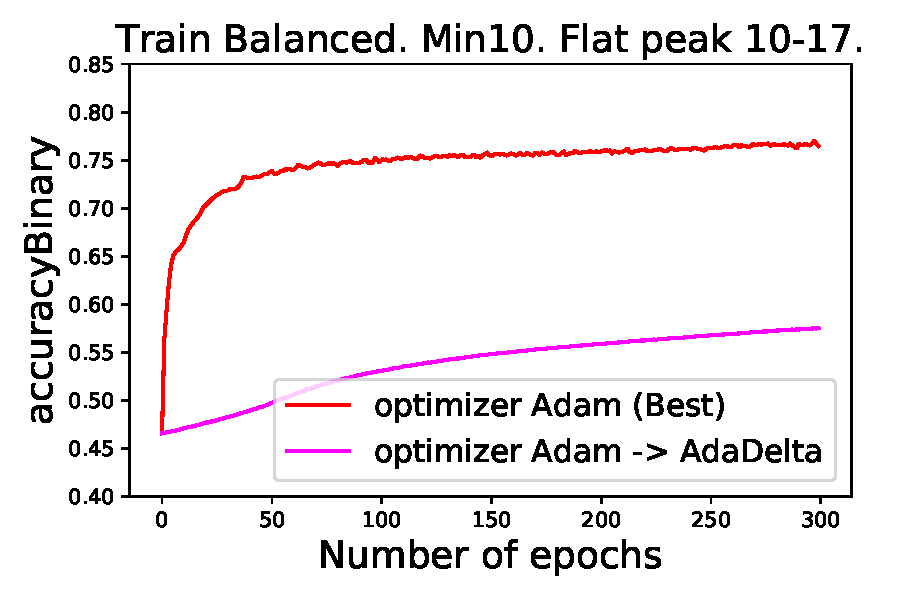
\includegraphics[width=0.32\textwidth]{plots/plot_01_1_overlay_graph_accuracyBinary_Train_Optimizer.pdf}
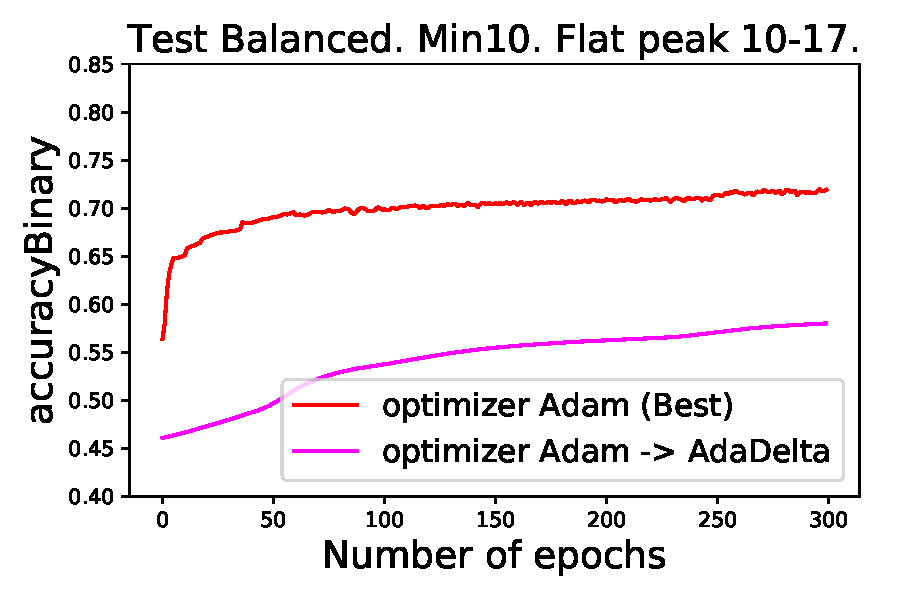
\includegraphics[width=0.32\textwidth]{plots/plot_01_1_overlay_graph_accuracyBinary_Test_Optimizer.pdf}\\
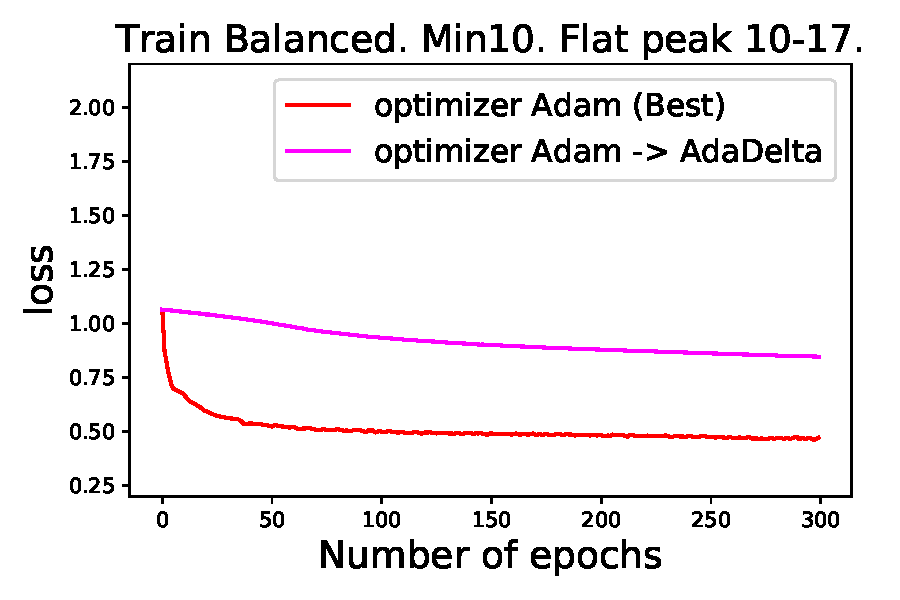
\includegraphics[width=0.32\textwidth]{plots/plot_01_1_overlay_graph_loss_Train_Optimizer.pdf}
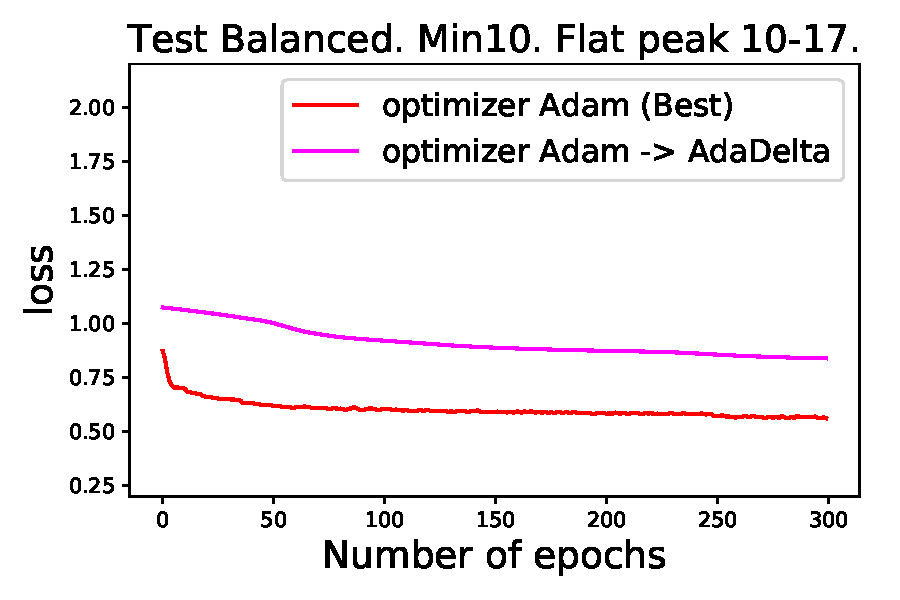
\includegraphics[width=0.32\textwidth]{plots/plot_01_1_overlay_graph_loss_Test_Optimizer.pdf}\\
\caption{Comparison of Adam and AdaDelta optimizers for the learning method. Adam is used in the final model. Binary accuracy and loss in Train and Test balanced samples.}
\label{fig:HPOptimizer}
\end{figure}

\ \\A comparison of the loss functions used to learn the weights and biases of the DNN via gradient descent, regular hinge and squared hinge, is studied. Their performance is similar, so the standard and mostly used regular hinge is retained for the final model, as illustrated in Figure~\ref{fig:HPLossFunction}.

\begin{figure}[!htb]
\centering
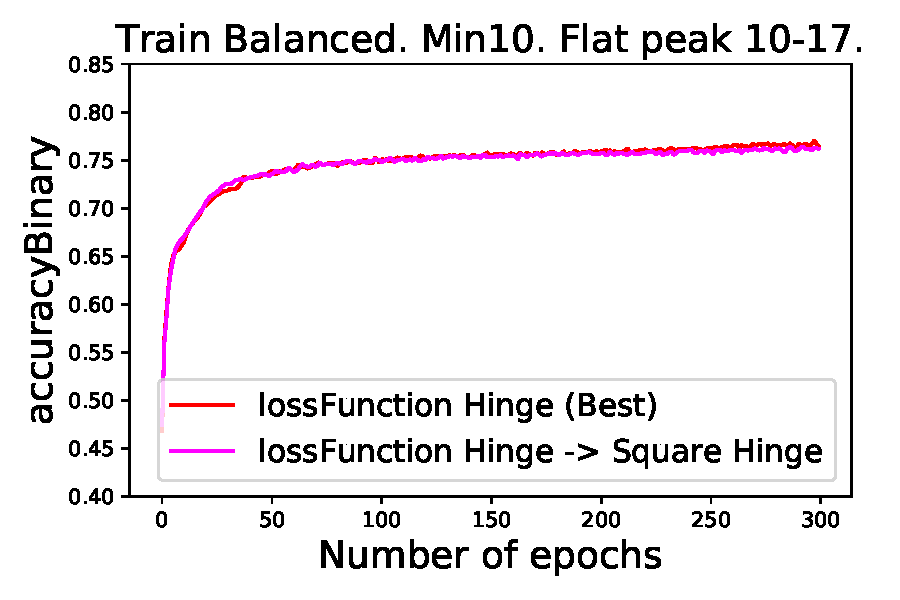
\includegraphics[width=0.32\textwidth]{plots/plot_01_1_overlay_graph_accuracyBinary_Train_LossFunction.pdf}
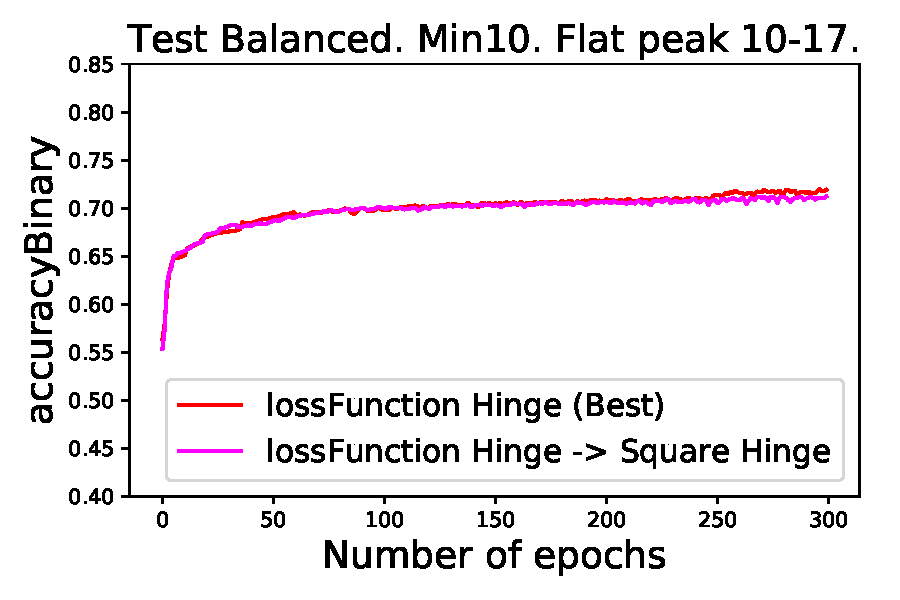
\includegraphics[width=0.32\textwidth]{plots/plot_01_1_overlay_graph_accuracyBinary_Test_LossFunction.pdf}\\
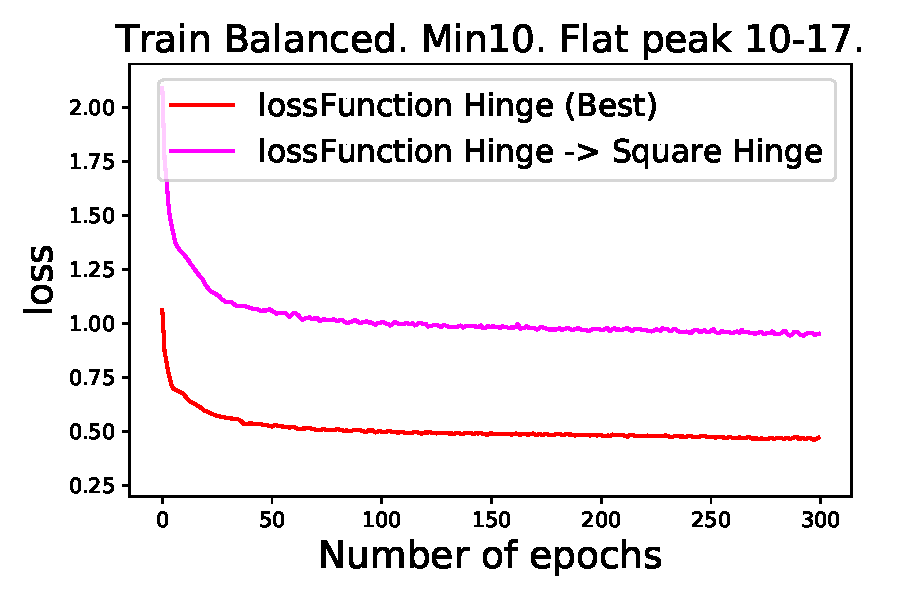
\includegraphics[width=0.32\textwidth]{plots/plot_01_1_overlay_graph_loss_Train_LossFunction.pdf}
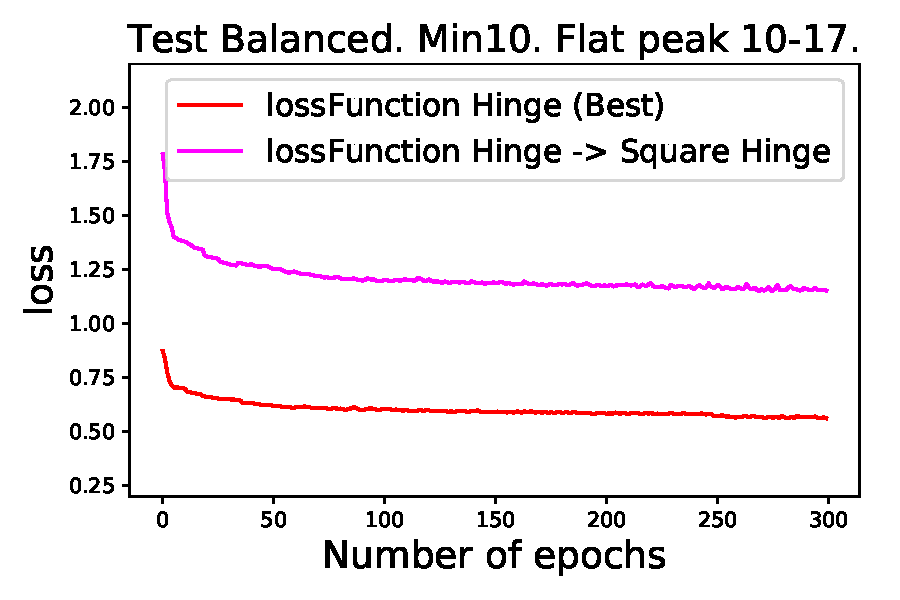
\includegraphics[width=0.32\textwidth]{plots/plot_01_1_overlay_graph_loss_Test_LossFunction.pdf}\\
\caption{Comparison of regular and square hinge loss functions for DNN learning. Regular hinge is used in the final model. Binary accuracy and loss in Train and Test balanced samples.}
\label{fig:HPLossFunction}
\end{figure}

\ \\The conclusion is that the learning part of the hyper-parameters tuning by comparing various batch sizes. The best performance is obtained for 50000, which is retained for the final model, as illustrated in Figure~\ref{fig:HPBatchSize}.

\begin{figure}[!htb]
\centering
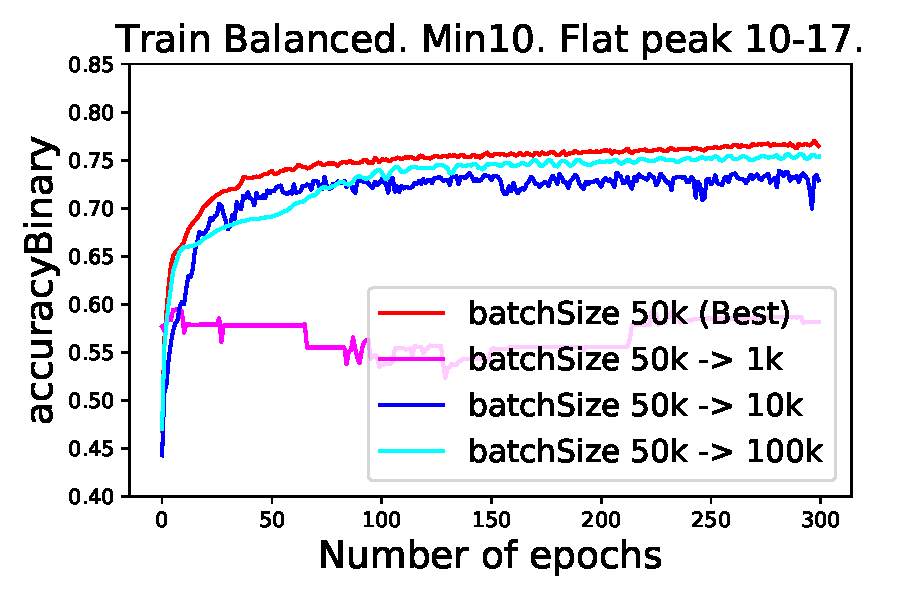
\includegraphics[width=0.32\textwidth]{plots/plot_01_1_overlay_graph_accuracyBinary_Train_BatchSize.pdf}
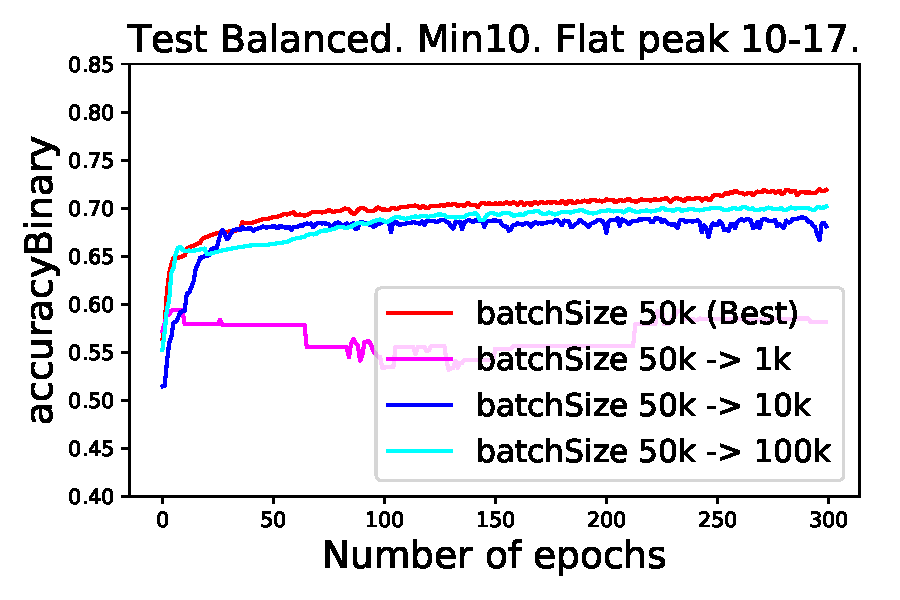
\includegraphics[width=0.32\textwidth]{plots/plot_01_1_overlay_graph_accuracyBinary_Test_BatchSize.pdf}\\
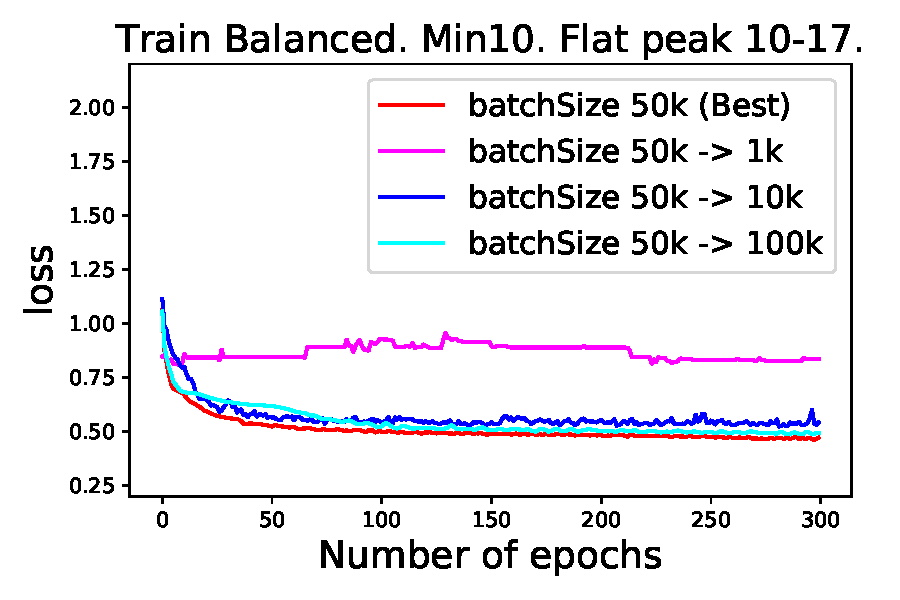
\includegraphics[width=0.32\textwidth]{plots/plot_01_1_overlay_graph_loss_Train_BatchSize.pdf}
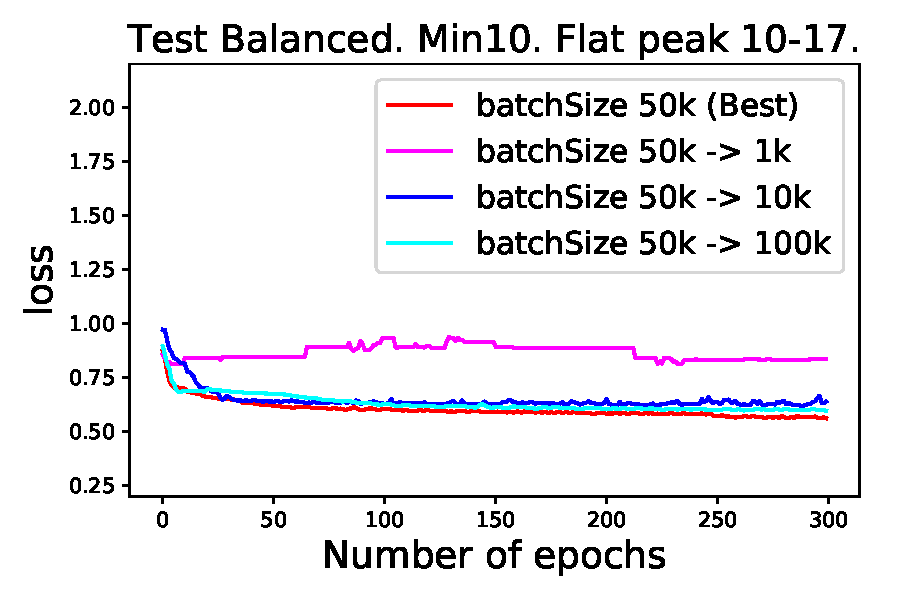
\includegraphics[width=0.32\textwidth]{plots/plot_01_1_overlay_graph_loss_Test_BatchSize.pdf}\\
\caption{Comparison of various batch sizes for DNN learning. A batch size of 50000 is used in the final model. Binary accuracy and loss in Train and Test balanced samples.}
\label{fig:HPBatchSize}
\end{figure}

\subsection{Best Model}
\label{sec:BestModel}

The problem structure fixes the number of nodes on the input layer to 60 (3 coordinates for 20 hits), and of the output layer to 20 (1 boolean for 20 hits). The DNN architecture and learning methods are optimised as hyper-parameters, whose options are limited by the choice of representing the answers yes and no by 1.0 and -1.0, respectively. The hyper-parameters that describe the best model are summarised as follows.

\ \\There are 3 hidden layers, each with 200 nodes, or 10 times more than the number of nodes in the output layer. A reminder is that the input layer has 60 nodes (3 coordinates x, y, z for each of the 20 hits in the bucket) and the output layer has 20 nodes (an output of -1.0 or 1.0 for each of the 20 hits in the bucket). A dropout layer (0.2) is added at the end of the hidden layers. The activation function for the hidden layers is the rectified linear unit (ReLU). The activation function for the last layer is hyperbolic tangent ($\tanh$). The loss function is the (regular) hinge function. The batch size is 50000.

\ \\While the choice of hyper-parameters is done using 300 epochs and the balanced test dataset, the final result uses 1200 epochs and the unbalanced test dataset.

\section{Predicting or Inference and Figures of Merit}

Once the model is trained, it can be applied to a new dataset to infer or make a prediction.

\ \\Besides the value of the loss function across the entire dataset, there is also another figure of merit of how well does a NN perform in training and testing. It is called \emph{accuracy} and is related to the number of of true positives or false negatives. The larger the accuracy, the better.

\ \\For the training dataset, the loss and accuracy values always improve. But in the testing dataset they can start to degrade if we train for too many epochs. By degrading it means that the loss value starts to grow, and the accuracy value starts to decrease. That is called over-training and consists of memorizing the inputs, and thus not being able to predict correctly any more for new inputs.

\ \\The confusion matrix is a table that summarises the performance of a binary classification model, as illustrated in Table~\ref{tab:ConfusionMatrix}. 

\begin{table}[h!]
 \centering
   
    \begin{tabular}{|l|l|} % <-- Alignments: 1st column left, 2nd middle and 3rd right, with vertical lines in between
      \hline
      TP & FP \\
      \hline
      FN & TN \\
      \hline
    \end{tabular}
\caption {Confusion Matrix.}
\label{tab:ConfusionMatrix}
\end{table}

\ \\The four metrics presented in the table are true positive (TP), false positive (FP), false negative (FN), and true negative (TN). Based on these four numbers further figures of merit are derived.

\ \\The accuracy defines what percentage of the total predictions are classified correctly, either as TP or TN, as defined by the Equation

\begin{equation}
   \Accuracy = \frac{\TP + \TN}{\TP + \TN + \FP + \FN}.
\end{equation}

\ \\The precision defines the percentage of the predicted positive that are actually positive, as defined by Equation

\begin{equation}
   \Precision = \frac{\TP}{\TP + \FP}.
\end{equation}

\ \\The recall defines the percentage of actual positive that are correctly predicted, as defined by the Equation

\begin{equation}
   \Recall = \frac{\TP}{\TP + \FN}.
\end{equation}

\ \\ The equivalents of the precision and recall can be constructed also for the negative values, as if the negative values are the sought target. The negative predicted value is the negative equivalent of precision and it represents the percentage of the predicted negative that in reality are also negative, as defined by the Equation

\begin{equation}
   \NegativePredictedValue = \frac{\TN}{\TN + \FN}.
\end{equation}

\ \\The true negative rate is the negative equivalent of the recall. It defines the percentage of the real negative that are also predicted as negative, as defined by the Equation 

\begin{equation}
   \TrueNegativeRate = \frac{\TN}{\TN + \FP}.
\end{equation} 

\ \\The pseudo-code to calculate the metrics is described in Appendix~\ref{sec:AppendixModelEvaluationMetrics}. 

\section{Software Used}

Several software Python libraries are used to perform this study, including data manipulation, the NN training, the figure of merit evaluation and plotting.

\ \\Numpy is a Python programming library, which is a coding support for large multi-dimensional arrays and matrices~\cite{Numpy}. 

\ \\PANDAS is a data manipulation and analysis library~\cite{PANDAS}. It is an open source library that is made mainly for working with relational or labeled data. It provides various data structures and operations for manipulating numerical data and time series. It is fast, has high performance and productivity. Data frames is a two-dimensional data structure with labeled data (rows and columns). Pandas uses numpy behind the hood. 

\ \\Jupyter Notebook is an important tool in the data science field. It is a web-based interactive computing platform~\cite{JupyterNotebook}. The Notebook combines code, equations, text, visualisation, interactive dashboard and other media. It works in line code, using blocks. 

\ \\Matplotlib is used for producing the plots in this thesis, both 1D and 2D~\cite{Matplotlib}.


